\begin{figure}[H]
	\begin{center}
		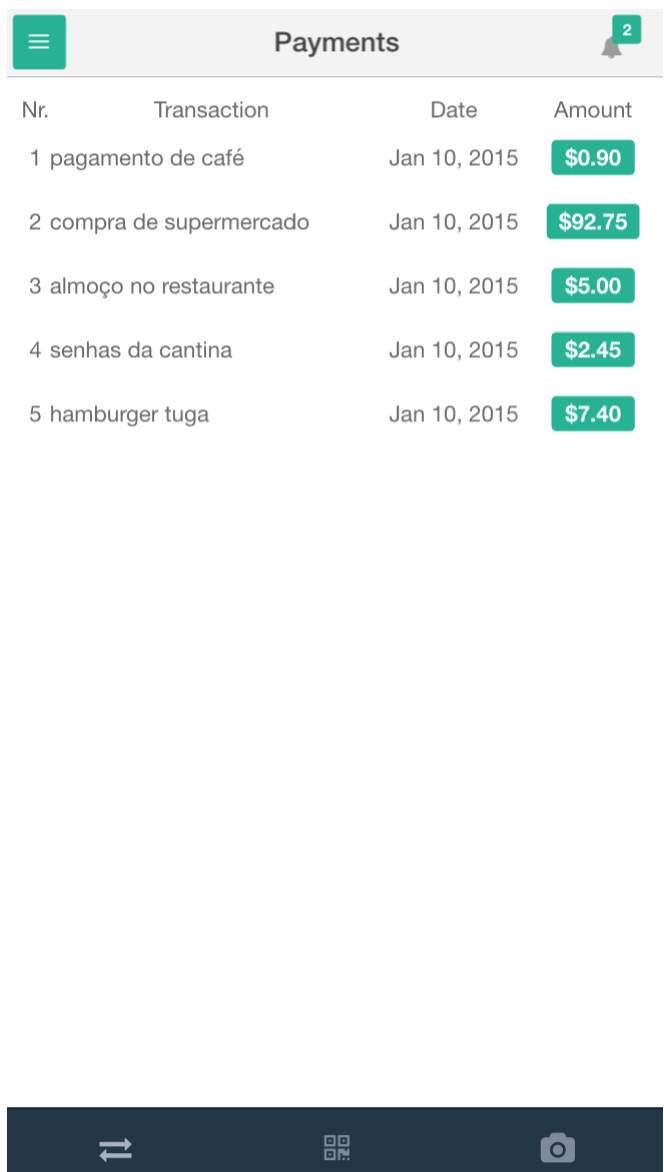
\includegraphics[width=0.5
		\textwidth]{payments/payments.png}
	\end{center}
	\caption{Pagamentos}
	\label{fig:4}
\end{figure}

\begin{figure}[H]
	\begin{center}
		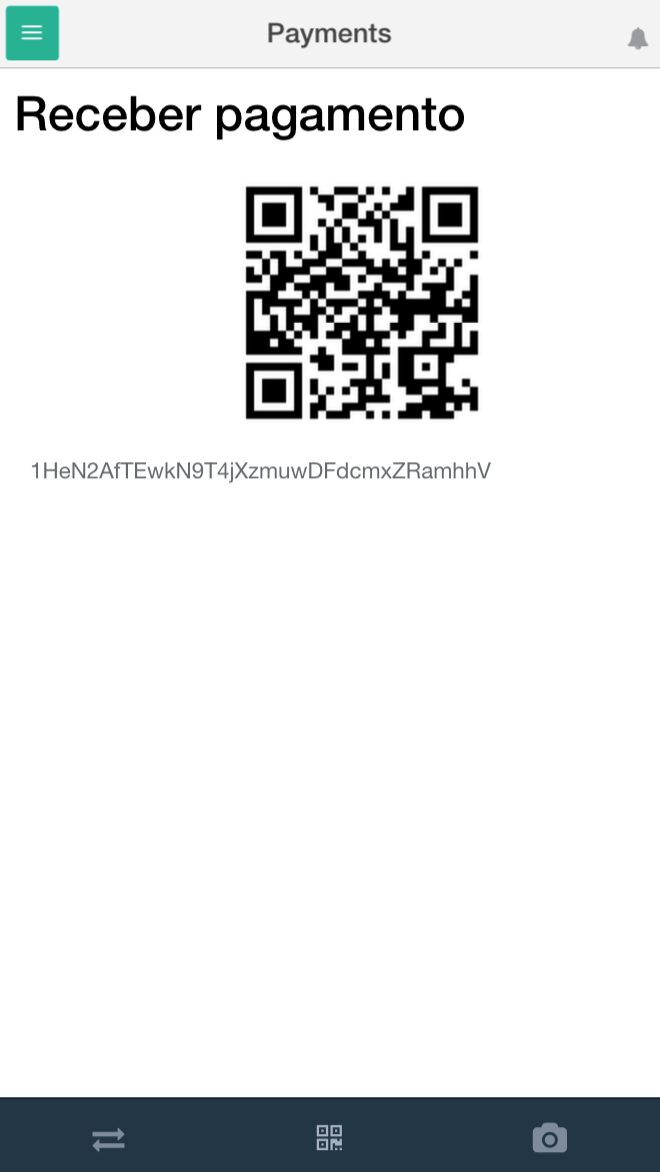
\includegraphics[width=0.5
		\textwidth]{payments/receive.png}
	\end{center}
	\caption{Receber Pagamento}
	\label{fig:4_1}
\end{figure}

O ecrã de pagamentos apresenta uma barra de navegação com três opções que se encontra no rodapé (ver Figura \ref{fig:4}). A primeira opção apresenta a lista de pagamentos, a segunda opção contém o \textit{QrCode} e o endereço \textit{bitcoin} para o utilizador receber dinheiro de outra pessoa (ver Figura \ref{fig:4_1}) e a terceira opção contém a opção de pagamento (ver Figura \ref{fig:4_2}).


\begin{figure}[H]
	\begin{center}
		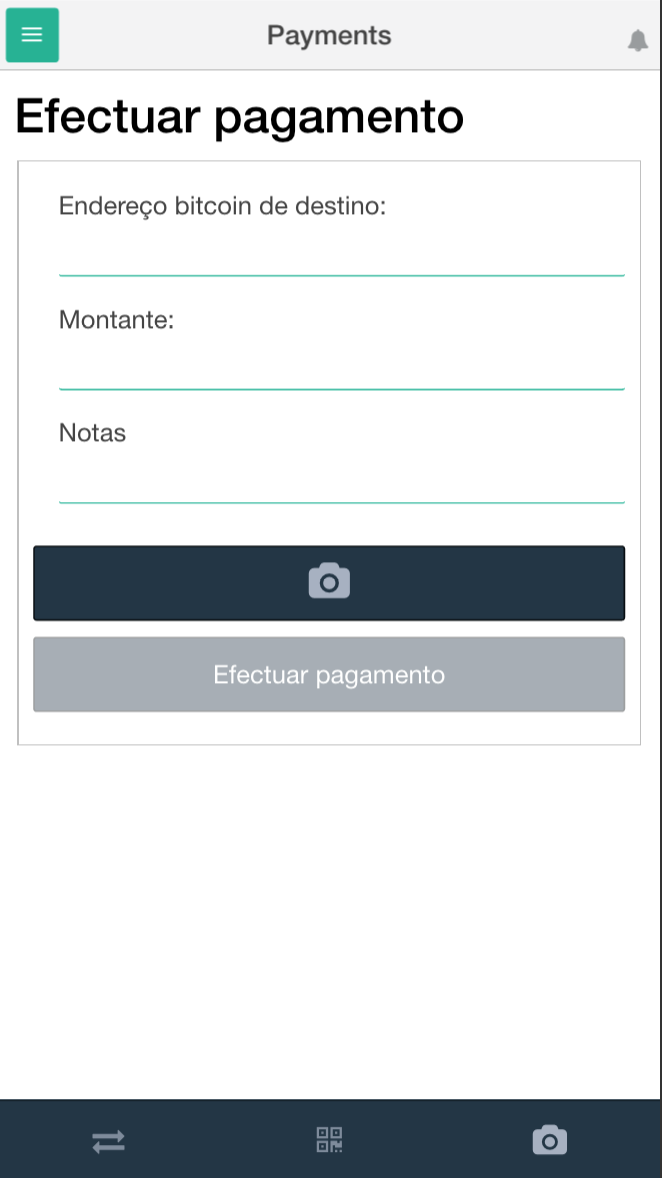
\includegraphics[width=0.5
		\textwidth]{payments/pay.png}
	\end{center}
	\caption{Pagar Despesa}
	\label{fig:4_2}
\end{figure}

 Na opção de pagamento é necessário inserir o endereço \textit{bitcoin} (ou usar o botão da câmara para obter o endereço através de um \textit{QrCode}), o montante a pagar e notas adicionais caso necessário.